\documentclass{article}
\usepackage[german]{babel}
\usepackage{float}
\usepackage{fourier}
\usepackage[utf8]{inputenc}
\usepackage[T1]{fontenc}
\usepackage{amsfonts,amsthm, amsmath}
\usepackage{listings}
% The following is needed in order to make the code compatible
% with both latex/dvips and pdflatex.
\ifx\pdftexversion\undefined
\usepackage[dvips]{graphicx}
\else
\usepackage[pdftex]{graphicx}
\DeclareGraphicsRule{*}{mps}{*}{}
\fi

\setlength\parindent{0pt}
\lstset{language=Erlang}

\begin{document}

\textbf{Team:} TEAM 01, Falco Winkler (FW), Daniel Schruhl (DS)\\
\\
\textbf{Aufgabenteilung:}
\begin{itemize}
    \item DLQ (DS)
    \item CMEM (DS)
	\item HBQ (FW)
	\item Server (DS)
\end{itemize}

\textbf{Quellenangaben:}\\
\\
\textbf{Bearbeitungszeitraum:}
\begin{itemize}
	\item 26.03.2017 (FW,DS)
	\item 03.04.2017 (DS)
	\item 04.04.2017 (DS)
	\item 05.04.2017 (FW,DS)
\end{itemize}

\textbf{Aktueller Stand:}
\begin{itemize}
	\item DLQ fertig und getestet
	\item CMEM fertig und getestet
	\item HBQ angefangen
	\item Server fertig
	\item Client
\end{itemize}

\textbf{Änderung des Entwurfs:}
\begin{itemize}
    \item Formatierung angepasst
	\item Komponentendiagramm erweitert
	\item Detailbeschreibungen für jedes Modul und Paket
\end{itemize}

\newpage

\section{Einführung und Ziele}
Es soll eine Message of the Day Anwendung erstellt werden. Dabei werden von verschiedenen Clients an einen Server verschiedene Nachrichten des Tages gesendet. Die Clients rufen vom Server alle Nachrichten ab, so dass jeder Client alle Nachrichten in einer festen Reihenfolge hat.

\subsection{Randbedingungen}
Es soll eine Client/Server-Architektur implementiert werden.
Der Server verwaltet dabei die ihm von den Clients gesendeten Nachrichten. Das beinhaltet eine feste Numerierung der Nachrichten.

Die Clients rufen dabei in bestimmten Abständen die Nachrichten ab. Falls ein Client dem Server schon bekannt ist, bekommt der nur die ihm noch unbekannten (neuen) Nachrichten.

Der Server muss sich also die Clients merken. Es soll mit einer Holdbackqueue und einer Deliveryqueue gearbeitet werden, um die korrekte Auslieferung in einer bestimmten Reihenfolge der Nachrichten zu garantieren.

\subsection{Kontextbegrenzung}
Das System soll in Erlang umgesetzt werden. Es muss auf Computern mit Linux Betriebssystem lauffähig sein.

\newpage

\section{Gesamtsystem}

\subsection{Bausteinsicht}
Das Softwareprodukt besteht aus mehreren Modulen und Paketen (Abbildung \ref{fig:component-diagram}). Diese Pakete setzen sich zusammen aus dem Client-Paket und dem Server-Paket.

\begin{figure}[H]
    \centering
    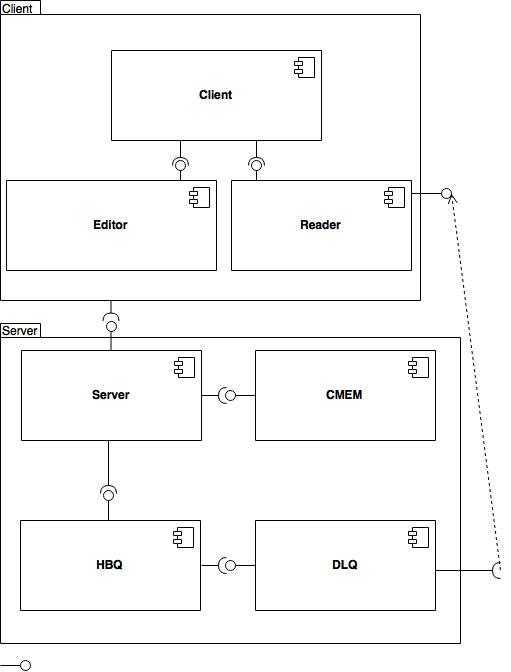
\includegraphics[width=0.5\textwidth]{component-diagram.png}
    \caption[seq-dia]{Komponentendiagramm der Message Of The Day App}
    \label{fig:component-diagram}
\end{figure}

Das Server Paket beinhaltet das Server-Modul und alle vom Server-Modul verwendeten Datenstrukturen.\\
Das Server-Modul ist für alle Funktionalitäten des Servers zuständig. Dazu gehört das Nummerieren und Verwalten der Nachrichten und die Verwaltung der Clients.\\
Das Server-Modul benutzt daher per Schnittstelle das HBQ-Modul und das CMEM-Modul. Das Server-Modul stellt eine Schnittstelle für die Clients bereit.\\
\\
Das CMEM-Modul ist für die Speicherung der Clients und ihrer aktuellen zu erwartenden Nachrichten Nummer zuständig. Das CMEM-Modul soll als lokale ADT realisiert werden. Diese wird nur vom Server angesprochen.\\
\\
Das HBQ-Modul ist für die Holdbackqueue zuständig und regelt die Sortierung der einkommenden Nachrichten in die Deliveryqueue und der damit verbundenen Fehlerbehandlung. Dabei ist das HBQ-Modul als entfernte ADT realisiert. Diese wird nur von dem Server-Modul verwendet.\\
\\
Das DLQ-Modul realsiert die Deliveryqueue, die für die Auslieferung der Nachrichten in Reihenfolge an die Clients zuständig ist. Die Schnittstelle des DLQ-Moduls wird nur vom HBQ-Modul konsumiert.\\
\\
Das Client-Paket beinhaltet die Client-Module. Diese sind zum einen der Lese Client (Reader-Modul) und der Redakteur Client (Editor-Modul). Beide Clients sind als ein Prozess implementiert und verwenden die vom Server bereitgestellte Schnittstelle. Der Redakteur Client ist für das Schicken von Nachrichten zuständig und der Lese Client für das Lesen von Nachrichten.

\subsection{Laufzeitsicht}
\begin{figure}[H]
\centering
\includegraphics[width=\textwidth]{sequence-diagram.png}
\caption[seq-dia]{Sequenzdiagramm bei fehlerfreiem Nachrichtenaustausch}
\label{fig:sequence-diagram}
\end{figure}

\newpage

\section{Subsysteme und Komponenten}
Das Server Modul und das Client Modul sind über Konfigurationsdateien konfigurierbar. Der Server, der Client und die HBQ
stellen Prozesse dar, die nebenläufig laufen. Dabei schreiben sie Log-Dateien, in denen ihre jeweiligen Aktionen
protokolliert werden.

\subsection{Server-Modul}
\subsubsection{Aufgabe und Verantwortung}
Der Server hat die Aufgabe Nachrichten von Clients entgegen zu nehmen, diese zu verarbeiten und an seine Subprozesse
bzw. an seine an ihn verbundenen Module weiter zu schicken. Der Server ist außerdem die zentrale Stelle für die
Koordinierung der nächst höchsten freien Nachrichtennummer, die von den Clients zum Senden verwendet werden soll.
Clients holen sich über den Server Nachrichten. Der Server reicht diese Anfragen an die relevanten Subprozesse weiter.

Wenn der Server für eine bestimmte Zeit von keinem Client mehr angesprochen wird, soll er sich und seine Subprozesse
herunterfahren.

\subsubsection{Schnittstelle}
\begin{lstlisting}[language=erlang]
/* Abfragen einer Nachricht */
Server ! {self(), getmessages},
receive {reply,[NNr,Msg,TSclientout,TShbqin,TSdlqin,TSdlqout],Terminated}

/* Senden einer Nachricht */
Server ! {dropmessage,[INNr,Msg,TSclientout]},

/* Abfragen der eindeutigen Nachrichtennummer */
Server ! {self(),getmsgid}

/* Nur fuer interne Prozesse: Einleiten des Herunterfahrens */
Server ! terminate

/* Nur fuer interne Prozesse: Terminierungsprozess erfolgreich, fahre runter*/
Server ! {reply,ok}
\end{lstlisting}

\textbf{getmessages}: Fragt beim Server eine aktuelle Textzeile ab. self() stellt die Rückrufadresse des Leser-Clients dar. Als Rückgabewert erhält er eine für ihn aktuelle Textzeile (Zeichenkette) zugestellt (Msg) und deren eindeutige Nummer (NNr).
Zudem erhält er die Zeitstempel explizit (erstellt durch erlang:now(), TSclientout, TShbqin, TSdlqin, TSdlqout).
Mit der Variablen Terminated signailiert der Server, ob noch für ihn aktuelle Nachrichten vorhanden sind. Terminated == false bedeutet, es gibt noch weitere aktuelle Nachrichten, Terminated == true bedeutet, dass es keine aktuellen Nachrichten mehr gibt, d.h. weitere Aufrufe von getmessages sind nicht notwendig.\\

\textbf{dropmessage}: Sendet dem Server eine Textzeile (Msg), die den  Namen des aufrufenden Clients und seine aktuelle Systemzeit sowie ggf. irgendeinen Text beinhaltet, zudem die zugeordnete (globale) Nummer der Textzeile (INNr) und seine Sendezeit (erstellt mit erlang:now(), TSclientout).\\

\textbf{getmsgid}: Fragt beim Server die aktuelle Nachrichtenummer ab. self() stellt die Rückrufadresse des Redakteur-Clients dar. Als Rückgabewert erhält er die aktuelle und eindeutige Nachrichtennummer (Number).\\

\textbf{terminate}: Nur von internen Prozessen zu verwenden. Startet den Terminierungsprozess.\\

\textbf{{reply, ok}}: Nur von internen Prozessen zu verwenden. Signalisiert, dass alle Submodule und Prozesse des Servers
heruntergefahren wurden und der Server nun selber herunterfahren kann.\\

\subsubsection{Entwurfsentscheidungen}
Der Server wird mit einer Start Funktion hochgefahren. Diese Funktion startet den Server-Prozess und konfiguriert ihn
mit den Werten, die in der Config stehen. Außerdem initialisiert der Server dabei eine CMEM (interne ADT) und startet
den Prozess der HBQ (externe ADT als Prozess) und initalisiert diese.

Der Server-Prozess hat einen State. In diesem State wird die CMEM, die Config, eine Verbindung zur HBQ (ProzessID),
die nächste Nachrichtennummer für einen Client zum Senden, ein Timer und die Latenz gespeichert.

Der Timer ist so eingestellt, dass er nach dem Ablaufen der Latenzzeit dem Server benachrichtigt sich herunterzufahren
(terminate). Dabei werden die Subprozesse heruntergefahren bevor der Server herunterfährt.

Jedes mal, wenn ein Client den Server über seine Schnittstelle anspricht, wird der Timer abgebrochen und zurück auf die
initiale Latenzzeit gestellt.

Bevor Clients dem Server eine Nachricht schicken können, müssen sie vom Server eine aktuelle Nachritennummer abfragen,
die sie für die neue Nachricht verwenden können. Diese Nummer ist im State des Server gespeichert und wird dann an den
anfragenden Client übermittelt. Danach wird diese Nummer im State inkrementiert.

Eingehende Nachrichtenzeilen von Clients werden vom Server an die HBQ weitergeleitet. Dabei wird dem Nachrichtentext der
aktuelle Zeitstempel hinzugefügt.

Wenn ein Client nach Nachrichten am Server anfragt, wird im CMEM nachgeschaut welche Nachrichtennummer für den Client
als nächstes vorgesehen wird und die HBQ beauftragt, diese dem Client zu schicken. Die dabei zurück gegeben verschickte
Nachrichtennummer wird dann im CMEM für den Client geupdated. Falls jedoch eine dummy Nachricht zurück kommt
(Nachrichtennummer: -1) findet dieses Update nicht statt.
			
\subsubsection{Konfigurationsparameter}
\begin{enumerate}
    \item{Latenzzeit bestimmt die maximale Zeit die der Server ungenutzt läuft}
    \item{Lebenszeit des Clients bestimmt die Zeit, für die sich der Server einen Client merkt}
    \item{Namen für den Server Prozess}
    \item{Größe der Deliveryqueue}
\end{enumerate}

\newpage

\subsection{CMEM-Modul}
\subsubsection{Aufgabe und Verantwortung}
Dieses Modul hat die Aufgabe sich anfragende Clients, ihre letzte bekommene Nachrichtennummer und den letzten Zeitpunkt ihrer Anfrage zu merken.
Clients, die sich seit einiger Zeit (Konfigurationsparameter) nicht gemeldet haben, werden vom CMEM als neue Clients behandelt (vergessen).

Die gespeicherten Daten sind über die Schnittstelle des Moduls vom Server aus abrufbar.

\subsubsection{Schnittstelle}
\begin{lstlisting}[language=erlang]
/* Initialisieren des CMEM */
initCMEM(RemTime,Datei): Integer X Atom -> CMem

/* Speichern/Aktualisieren eines Clients in dem CMEM */
updateClient(CMEM,ClientID,NNr,Datei): Cmem X PID X Integer X Atom -> CMem

/* Abfrage welche Nachrichtennummer der Client als naechstes erhalten darf */
getClientNNr(CMEM,ClientID) : Cmem X PID -> Integer
\end{lstlisting}

\textbf{initCMEM(RemTime,Datei)}: initialisiert den CMEM. RemTime gibt dabei die Zeit an, nach der die Clients vergessen werden Bei Erfolg wird ein leeres CMEM zurück geliefert. Datei kann für ein logging genutzt werden.\\

\textbf{updateClient(CMEM,ClientID,NNr,Datei)}: speichert bzw. aktualisiert im CMEM den Client ClientID und die an ihn gesendete Nachrichtenummer NNr. Datei kann für ein logging genutzt werden.\\

\textbf{getClientNNr(CMEM,ClientID)}: gibt die als nächstes vom Client erwartete Nachrichtennummer des Clients ClientID aus CMEM zurück. Ist der Client unbekannt wird 1 zurück gegeben.\\

\subsubsection{Entwurfsentscheidungen}
Die CMEM wird mit Hilfe einer Liste realisiert. An erster Stelle der CMEM Liste steht die Liste der Clients. Die Elemente der Client Liste sind Tupel, die aus der Client Prozess ID, der zuletzt erhaltenen NNr und einem Timestamp der letzten Aktion in Millisekunden bestehen.

An zweiter Stelle der CMEM Liste steht die maximale Zeit, für die ein Client gemerkt wird in Millisekunden.

\begin{lstlisting}[language=erlang]
/* Client Tupel Format */
Client := {ClientPID,NNr,ClientTS}:
    {PID X Integer X Integer}

/* CMEM Format */
/* ClientList ist Liste bestehend aus Clients */
/* RemTime ist Zeit in Millisekunden fuer die Clients gemerkt werden */
CMEM := [ClientList, RemTime]: [List X Integer]
\end{lstlisting}

Falls beim Aktualisieren eines Clients der Client noch nicht im CMEM steht, wird er hinzugefügt.
Ansonsten wird er einfach mit den angegebenen Parametern in der CMEM Client Liste aktualisiert.\\

Wenn die nächste Nachrichtennummer für einen Client abgerufen wird (\texttt{getClientNNr}), wird ein Check gemacht, ob der Client bekannt ist.
Ein Client ist bekannt, wenn er in der CMEM Liste steht und wenn die Summe seines Timestamps mit der RemTime größer gleich der aktuellen Zeit (als Timestamp) ist.\\

Für bekannte Clients wird die resultierende nächste Nachrichtennummer inkrementiert. Für unbekannte Clients wird 1 als nächste Nachrichtennummer zurück gegeben.

\subsubsection{Konfigurationsparameter}
\begin{enumerate}
    \item{Zeit nach der die Clients vergessen werden in Millisekunden (RemTime)}
\end{enumerate}

\newpage
			
\subsection{Komponente HBQ}
\subsubsection{Aufgabe und Verantwortung der HBQ}
Von Redakteur-Clients gesendete Nachrichten werden hier zwischengespeichert. Gibt es keine Lücke in der fortlaufenden Nummerierung der Nachrichten, werden Sie an die DLQ weitergeleitet. Bei einer Überfüllung der HBQ (2/3 der Maximalen Kapazität der DLQ) wird die älteste Lücke in den Nachrichten mit einer künstlichen Nachricht geschlossen, und es werden erneut alle Lückenlosen Nachrichten an die DLQ weitergeleitet. Die HBQ stellt nur ein Interface für den Server bereit.

\subsubsection{Entwurfsentscheidungen}
Es wird die Aktuelle NNr gespeichert.
Jede Nachricht, die der aktuellen erwarteten NNr entspricht, wird direkt weitergeleitet.
Wenn noch auf alte Nachrichten gewartet wird, wird die nachricht in die HBQ eingefügt.
Wenn die Nachrichtennummer größer als der erwarteten Nachrichtennummer ist,
müssen alle bereits empfangenennachrichten ab der erwarteten Nachrichtennummer durchgegangen werden.
Die Nachrichten, die aufeinanderfolgende Sequenznummern haben oder eine Dummy Nachricht sind werden an die
DLQ ausgeliefert. 

Die Dummynachrichten schließen Lücken bestehend aus einer oder mehrerer Sequenznummern.
Eine Dummynachricht wird durch den String "Fehlernachricht" im Inhalt identifiziert.
Ihre NNr wird auf das Ende des Intervalls, welches Sie abdeckt festgelegt.

Die Liste wird nach jedem Einfügen Sortiert, um die Reihenfolge zu erhalten. Wenn die Liste überfüllt ist,
wird rekursiv die erste Lücke zwischen Sequenznummern gesucht. Dann wird eine entsprechende 
Dummy - Nachricht für diese Lücke eingefügt, und die Funktion zum Senden aller aufeinanderfolgenden Sequenznummern wird erneut aufgerufen.
So werden mindestens alle Nachrichten bis zum Abschluss der Lücke aus der HBQ entfernt.

				
\subsubsection{Außensicht}

\subsubsection{Innensicht}

\subsubsection{Konfigurationsparameter}
\begin{itemize}
	\item Die Maximalgröße der DLQ wird verwendet um die HBQ bei kritischer Überfüllung zu leeren.
\end{itemize}
\newpage

\subsection{DLQ-Modul}
\subsubsection{Aufgabe und Verantwortung}
Die Deliveryqueue hat die Aufgabe Nachrichten an Clients zuzustellen und stellt eine Datenstruktur dar, die eine
maximale Menge (Kapazität) an Nachrichten hält. Sie verhält sich dabei wie von einer Warteschlange zu erwarten beim
Einfügen und Herausholen von Nachrichten (FIFO). Nur das HBQ-Modul darf auf das DLQ-Modul zugreifen. Das DLQ-Modul
sendet über eine Schnittstelle der Clients die Nachrichten an die Clients.

In der DLQ sind die Nachrichten absteigend von vorne nach hinten sortiert.

\subsubsection{Schnittstelle}
\begin{lstlisting}[language=erlang]
/* Initialisieren der DLQ */
initDLQ(Size,Datei): Integer X Atom -> DQueue

/* Abfrage welche Nachrichtennummer in der DLQ gespeichert werden kann */
expectedNr(Queue) : DQueue -> Integer

/* Speichern einer Nachricht in der DLQ */
push2DLQ([NNr,Msg,TSclientout,TShbqin],Queue,Datei) :
    MSG_list X DQueue X Atom -> DQueue

/* Ausliefern einer Nachricht an einen Leser-Client */
deliverMSG(MSGNr,ClientPID,Queue,Datei):
    Integer X PID X DQueue X Atom -> Integer
\end{lstlisting}

\textbf{initDLQ(Size,Datei)}: initialisiert die DLQ mit Kapazität Size. Bei Erfolg wird eine leere DLQ zurück geliefert.
Datei kann für ein logging genutzt werden.\\

\textbf{expectedNr(Queue)}: liefert die Nachrichtennummer, die als nächstes in der DLQ gespeichert werden kann.
Bei leerer DLQ ist dies 1.\\

\textbf{push2DLQ([NNr,Msg,TSclientout,TShbqin],Queue,Datei)}: speichert die Nachricht [NNr,Msg,TSclientout,TShbqin] in
der DLQ Queue und fügt ihr einen Eingangszeitstempel an (einmal an die Nachricht Msg und als expliziten Zeitstempel
TSdlqin mit erlang:now() an die Liste an. Bei Erfolg wird die modifizierte DLQ zurück geliefert. Datei kann für ein
logging genutzt werden.\\

\textbf{deliverMSG(MSGNr,ClientPID,Queue,Datei)}: sendet die Nachricht MSGNr an den Leser-Client ClientPID. Dabei wird
ein Ausgangszeitstempel TSdlqout mit erlang:now() an das Ende der Nachrichtenliste angefügt. Sollte die Nachrichtennummer
nicht mehr vorhanden sein, wird die nächst größere in der DLQ vorhandene Nachricht gesendet. Bei Erfolg wird die
tatsächlich gesendete Nachrichtennummer zurück geliefert. Datei kann für ein logging genutzt werden.\\

\subsubsection{Entwurfsentscheidungen}
Die Deliveryqueue wird als Liste realisiert. Das erste Element der Liste ist dabei eine Liste der Nachrichten und das
zweite Element der Liste gibt die Kapazität der DLQ an.
\begin{lstlisting}[language=erlang]
/* Nachrichten Format */
/* minimal 3 Elemente, pro Station kommt eins hinzu; maximal 6 Elemente */
MSG_List := [NNr,Msg,TSclientout,TShbqin,TSdlqin]:
    [Integer X String X 3-Tupel X 3-Tupel X 3-Tupel]

/* DLQ Format */
/* Nachrichtenliste ist eine Liste aus MSG_List und hat */
/* maximal Kapazitaet Anzahl an Elementen */
DLQ := [Nachrichtenliste, Kapazitaet]: [List X Integer]
\end{lstlisting}

Neue Nachrichten werden am Anfang der Liste angefügt. Das vereinfacht die Nachfrage nach der nächsten zu speichernden
Nachrichtennummer in der DLQ. Das ist die Nachrichtennummer der ersten Nachricht in der DLQ um eins inkrementiert.

Demnach werden Nachrichten am Ende der Liste entnommen. Wenn eine Nachricht in die DLQ eingetragen wird, wird ans Ende
der Nachricht der aktuelle Zeitstempel zum Zeitpunkt des Einfügens hinzugefügt.

Beim Eintragen wird außerdem überprüft, ob die DLQ schon voll ist. Wenn die DLQ voll ist, wird die Nachricht am Ende der
DLQ gelöscht und die neue DLQ danach eingefügt (FIFO).\\

Beim Senden einer Nachricht durch Angabe der Nachrichtennummer wird in der DLQ nach der Nachricht mit der
Nachrichtennummer oder der nächst höchsten Nachrichtennummer gesucht.\\

Das finden der richtigen Nachricht übernimmt eine Hilfsfunktion. Diese bekommt die Nachrichtenliste der DLQ in
umgekehrter Reihenfolge. Dadurch hat diese Hilfsfunktion die Nachrichtenliste der DLQ in aufsteigender Reihenfolge.

Nun sucht die Hilfsfunktion innerhalb dieser Liste das erste vorkommen einer Nachricht mit der Nachrichtennummer größer
gleich der gewünschten Nachrichtennummer (von links nach rechts). Dadurch wird entweder die Nachricht mit der angefragten Nachrichtennummer
gefunden oder die Nachricht mit der nächst höchsten Nachrichtennummer.

Falls überhaupt keine passende Nachricht gefunden wird (DLQ leer / Nachrichtennummer zu groß), wird eine dummy Nachricht
zurückgegeben, die eine -1 als Nachrichtennummer hat. Dadurch kann sie als dummy Nachricht identifiert werden.\\

Die aus der Hilfsfunktion resultierende Nachricht wird mit einem Zeitstempel versehen. Beim Senden dieser Nachricht wird
die Nachricht zusammen mit einem boolean Flag an den Client gesendet. Dieses boolean Flag signalisiert, ob keine
weiteren Nachrichten folgen.

Dieses Flag ist wahr, wenn entweder eine Fehlernachricht vorliegt oder die Nachricht mit der Nachrichtennumer des ersten
Elementes der DLQ.

\subsubsection{Konfigurationsparameter}
\begin{itemize}
    \item Kapazität der DLQ als ganze Zahl
\end{itemize}

\end{document}